\hyphenation{diffe-rent}
%%%%%%%%%%%%%%%%%%%%% Conclusions %%%%%%%%%%%%%%%%%
\chapter{Conclusions}
\label{ch:Conclusions}

In this dissertation, a search for double Higgs boson production (HH) mediated by a KK graviton or a radion is presented. The double Higgs system subsequently decays through the intermediate $bbZZ$ state - one of the Higgs bosons decays to two b quarks, while the other decays to a pair of Z bosons, which, in turn, decay to a pair of neutrinos and a pair of electrons or muons. The search is performed in data samples corresponding to an integrated luminosity of 35.9 fb$^{-1}$ at $\sqrt s =13$ TeV, recorded by the CMS experiment at the LHC in 2016. 

This is the first search for a double Higgs boson production in the $bbZZ$ intermediate channel that was done at CERN. The double Higgs boson physics is an important test of the standard model and can open doors to the beyond the standard model physics. The HH process observed in a resonant production mode would mean new physics, while observed in non-resonant mode at the SM predicted level allows one to study Higgs boson self-coupling. 

No statistically significant deviations from the standard model theory predictions for background processes have been observed, and 95\% upper level confidence limits are reported for production cross section of a KK graviton or a radion times the branching fraction of its subsequent decay into a di-Higgs system, and further to the $2 b 2 \ell 2 \nu$ final state. The limits are derived for resonance masses in the 250 GeV to 1 TeV range.

This measurement has been approved by the CMS Collaboration and became public in November 2018. The measurement is part of an intensive program of the search for di-Higgs production in CMS in a wide range of channels. Current projections suggest that the first observation of this process, if no new physics is  found, is not expected by any individual HH channel. The CMS plan is to combine several HH channels. The first such combination was completed in early 2018, but did not include this measurement. The next step is to combine present CMS searches in $bbZZ$ channels, and then to add them to combination of all approved HH states. 

\clearpage

\section*{CERN guide, S'Cool Lab teacher, Finance Club admin, Boxing Club coach}
\small

It has been a great pleasure to stay at CERN for four years. From the bottom of my heart, I want to thank my adviser and my HEP group for such an opportunity. I have exploited all the possible areas of science, outreach, fun, and joy available at CERN. Well, almost all, and I know it is ridiculous or even silly, but here, in Gen\`eve, I have not tried skiing...

I have been an official CERN guide, giving people tours to the Antimatter Decelerator, the ATLAS control room, the Low Energy Ion Ring complex, the Proton Synchrotron, the LHC control room, the Data Centre, the SM18 facility (a world leading magnet test facility for testing magnets and instrumentation at low temperature and high currents), and the Alpha Magnetic Spectrometer control room. Audience ranged from middle school kids to emeritus professors of science. 

Also, I have been a teacher at the S'Cool Lab, where high school students have a chance to come to CERN and build at this ``cool'' scientific laboratory a real experimental setup and then conduct the experiment on their own. 

For more than a year I have been an administrative managing officer at the CERN Finance Club. I was responsible for inviting top professionals from the finance and fintech companies to give talks at our club. I started the ``quant group'' at the club and was the first to optimise our portfolio of stocks using Monte Carlo methods and also using the minimisation techniques. Needless to say, that would not be possible if I have not learnt those tools first in High Energy Physics!

Last but not least, my friends from the CERN Powerlifting Club introduced me to the Boxing Club. There is where I met most of my CMS and ATLAS friends. I have been training people with the goal to improve their health. As a side effect, some picked up self-defence, others had fun and found themselves truly addicted to this combination of the hard work and laughter. A few people even became very much into the world of the intelligent boxing, which is not about power, but about strategy and outworking the opponent \ref{outreach}. 


\iffalse

\begin{figure}[h]
     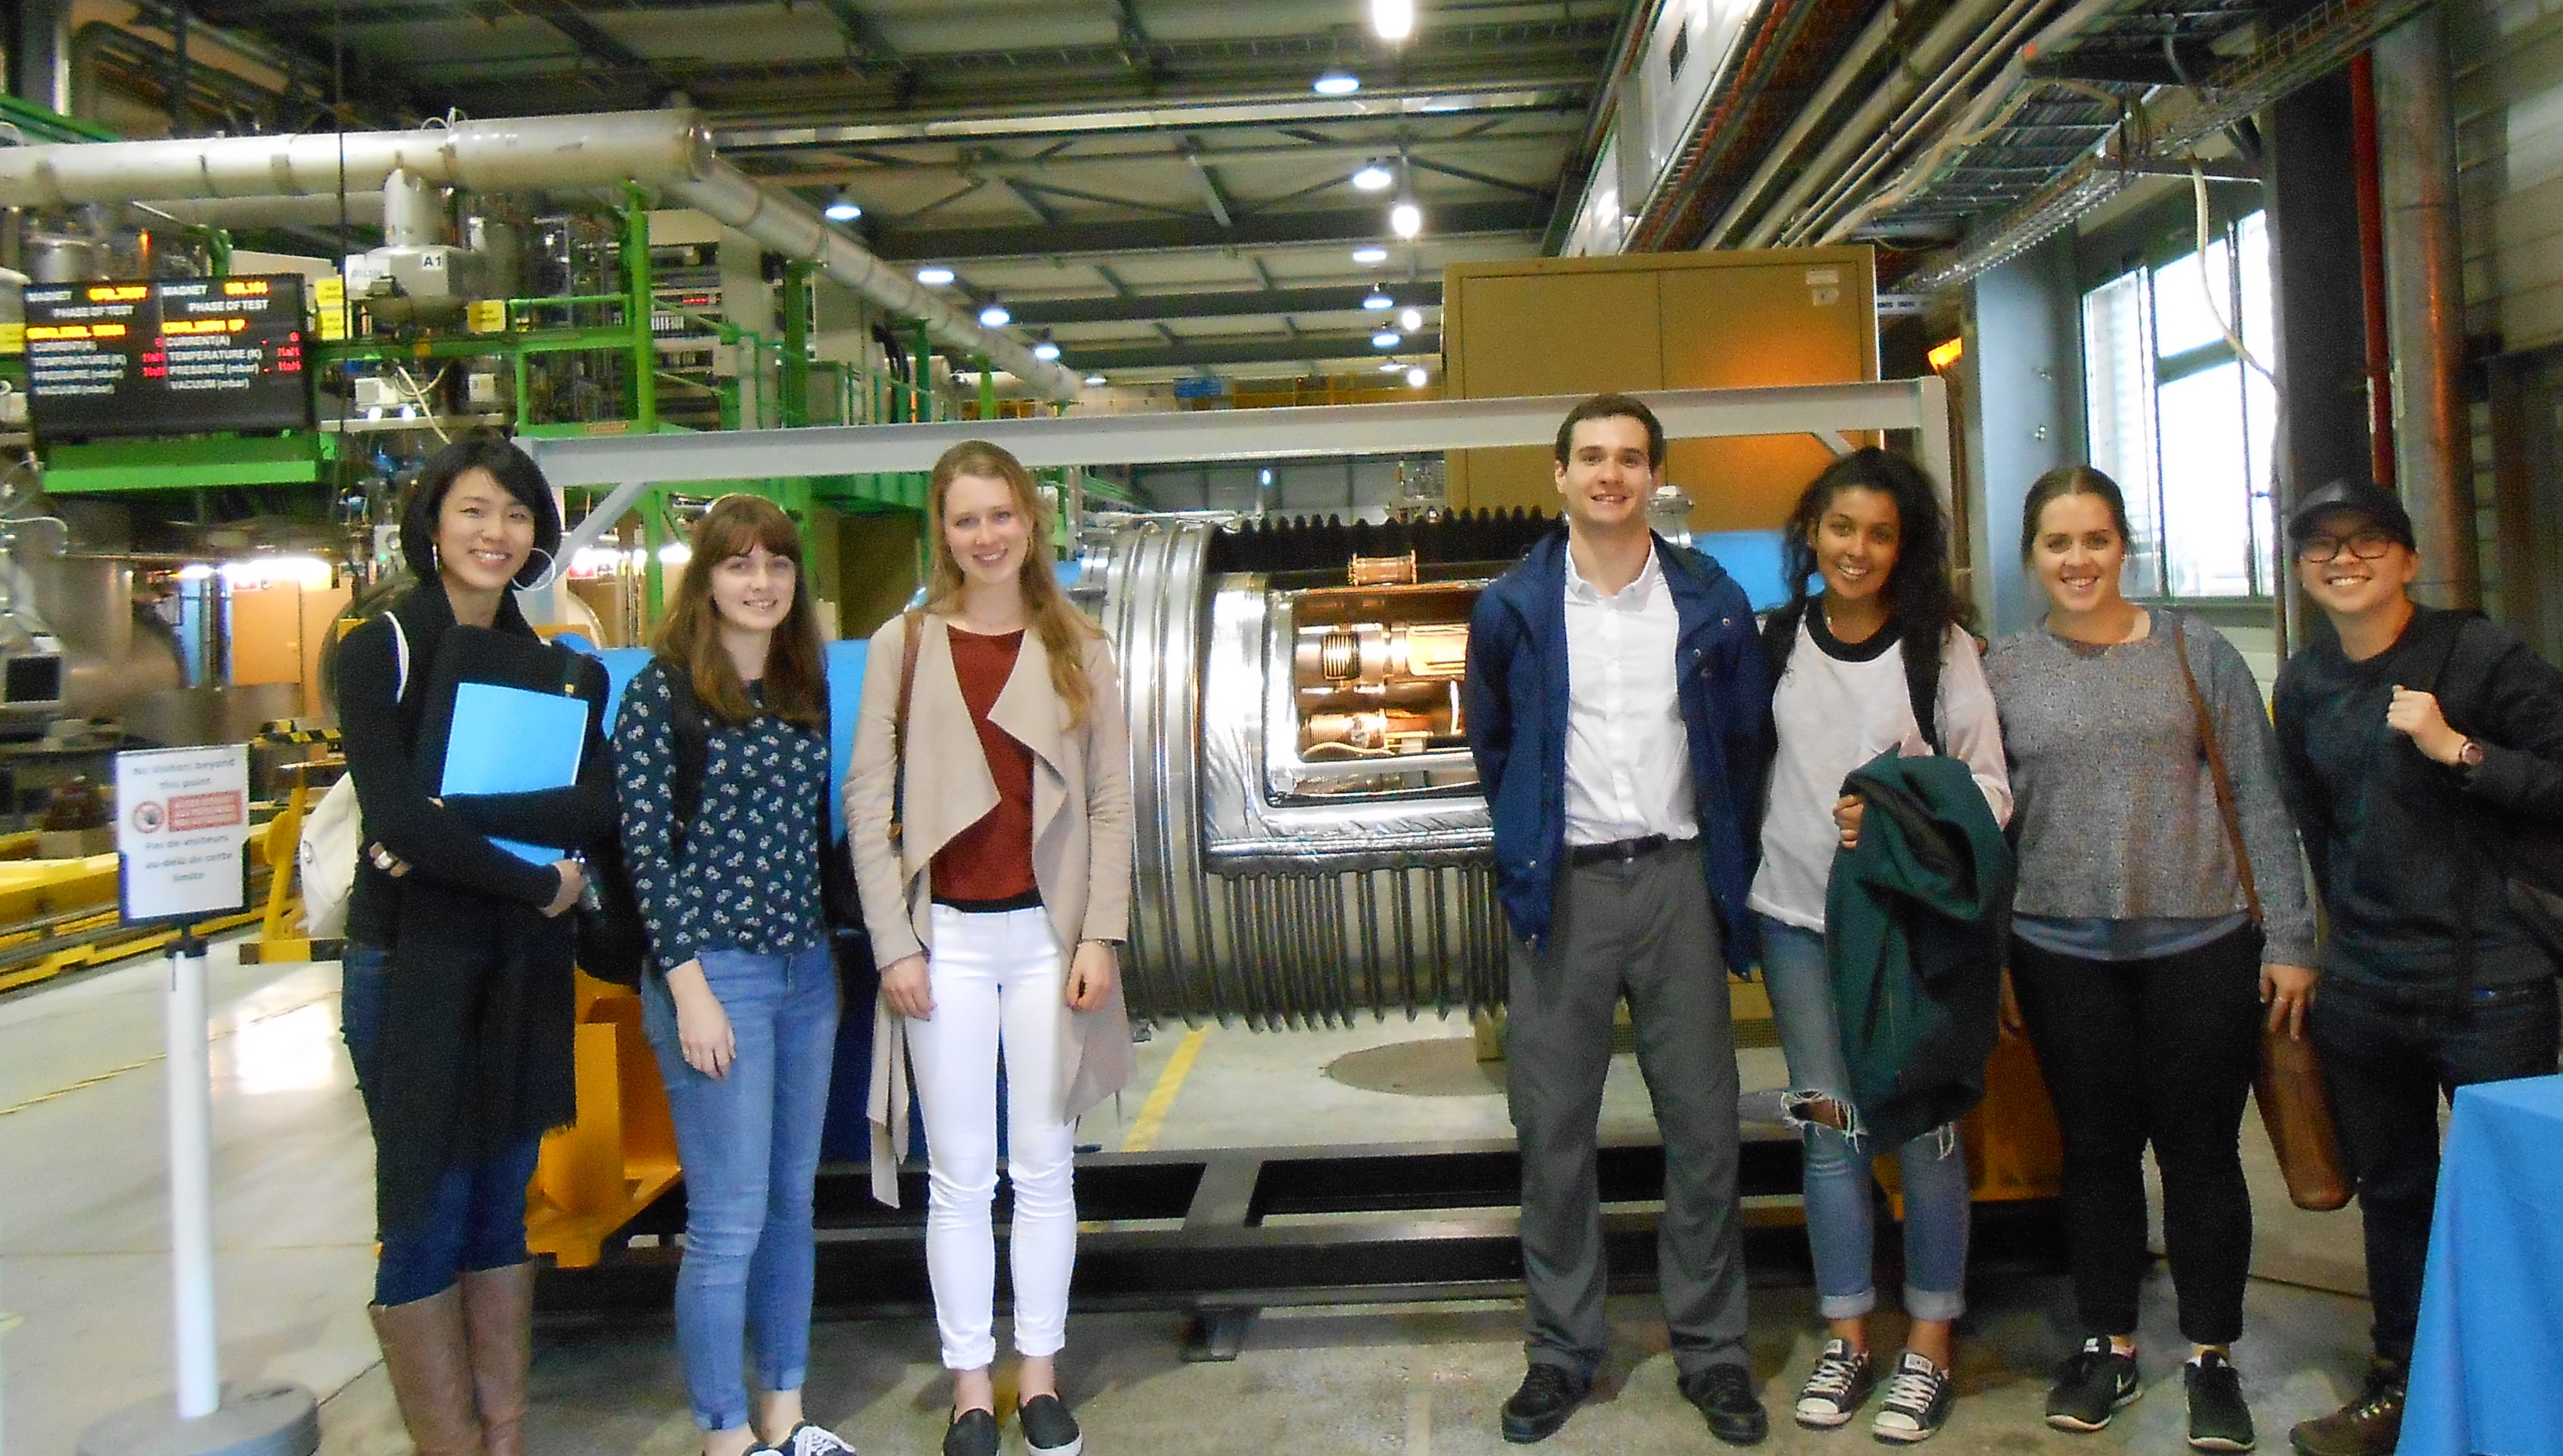
\includegraphics[width=0.54\textwidth]{uni_of_geneva}
     \includegraphics[width=0.54\textwidth]{scoollab3.png}\\
     \includegraphics[width=0.54\textwidth]{finance1.png}
     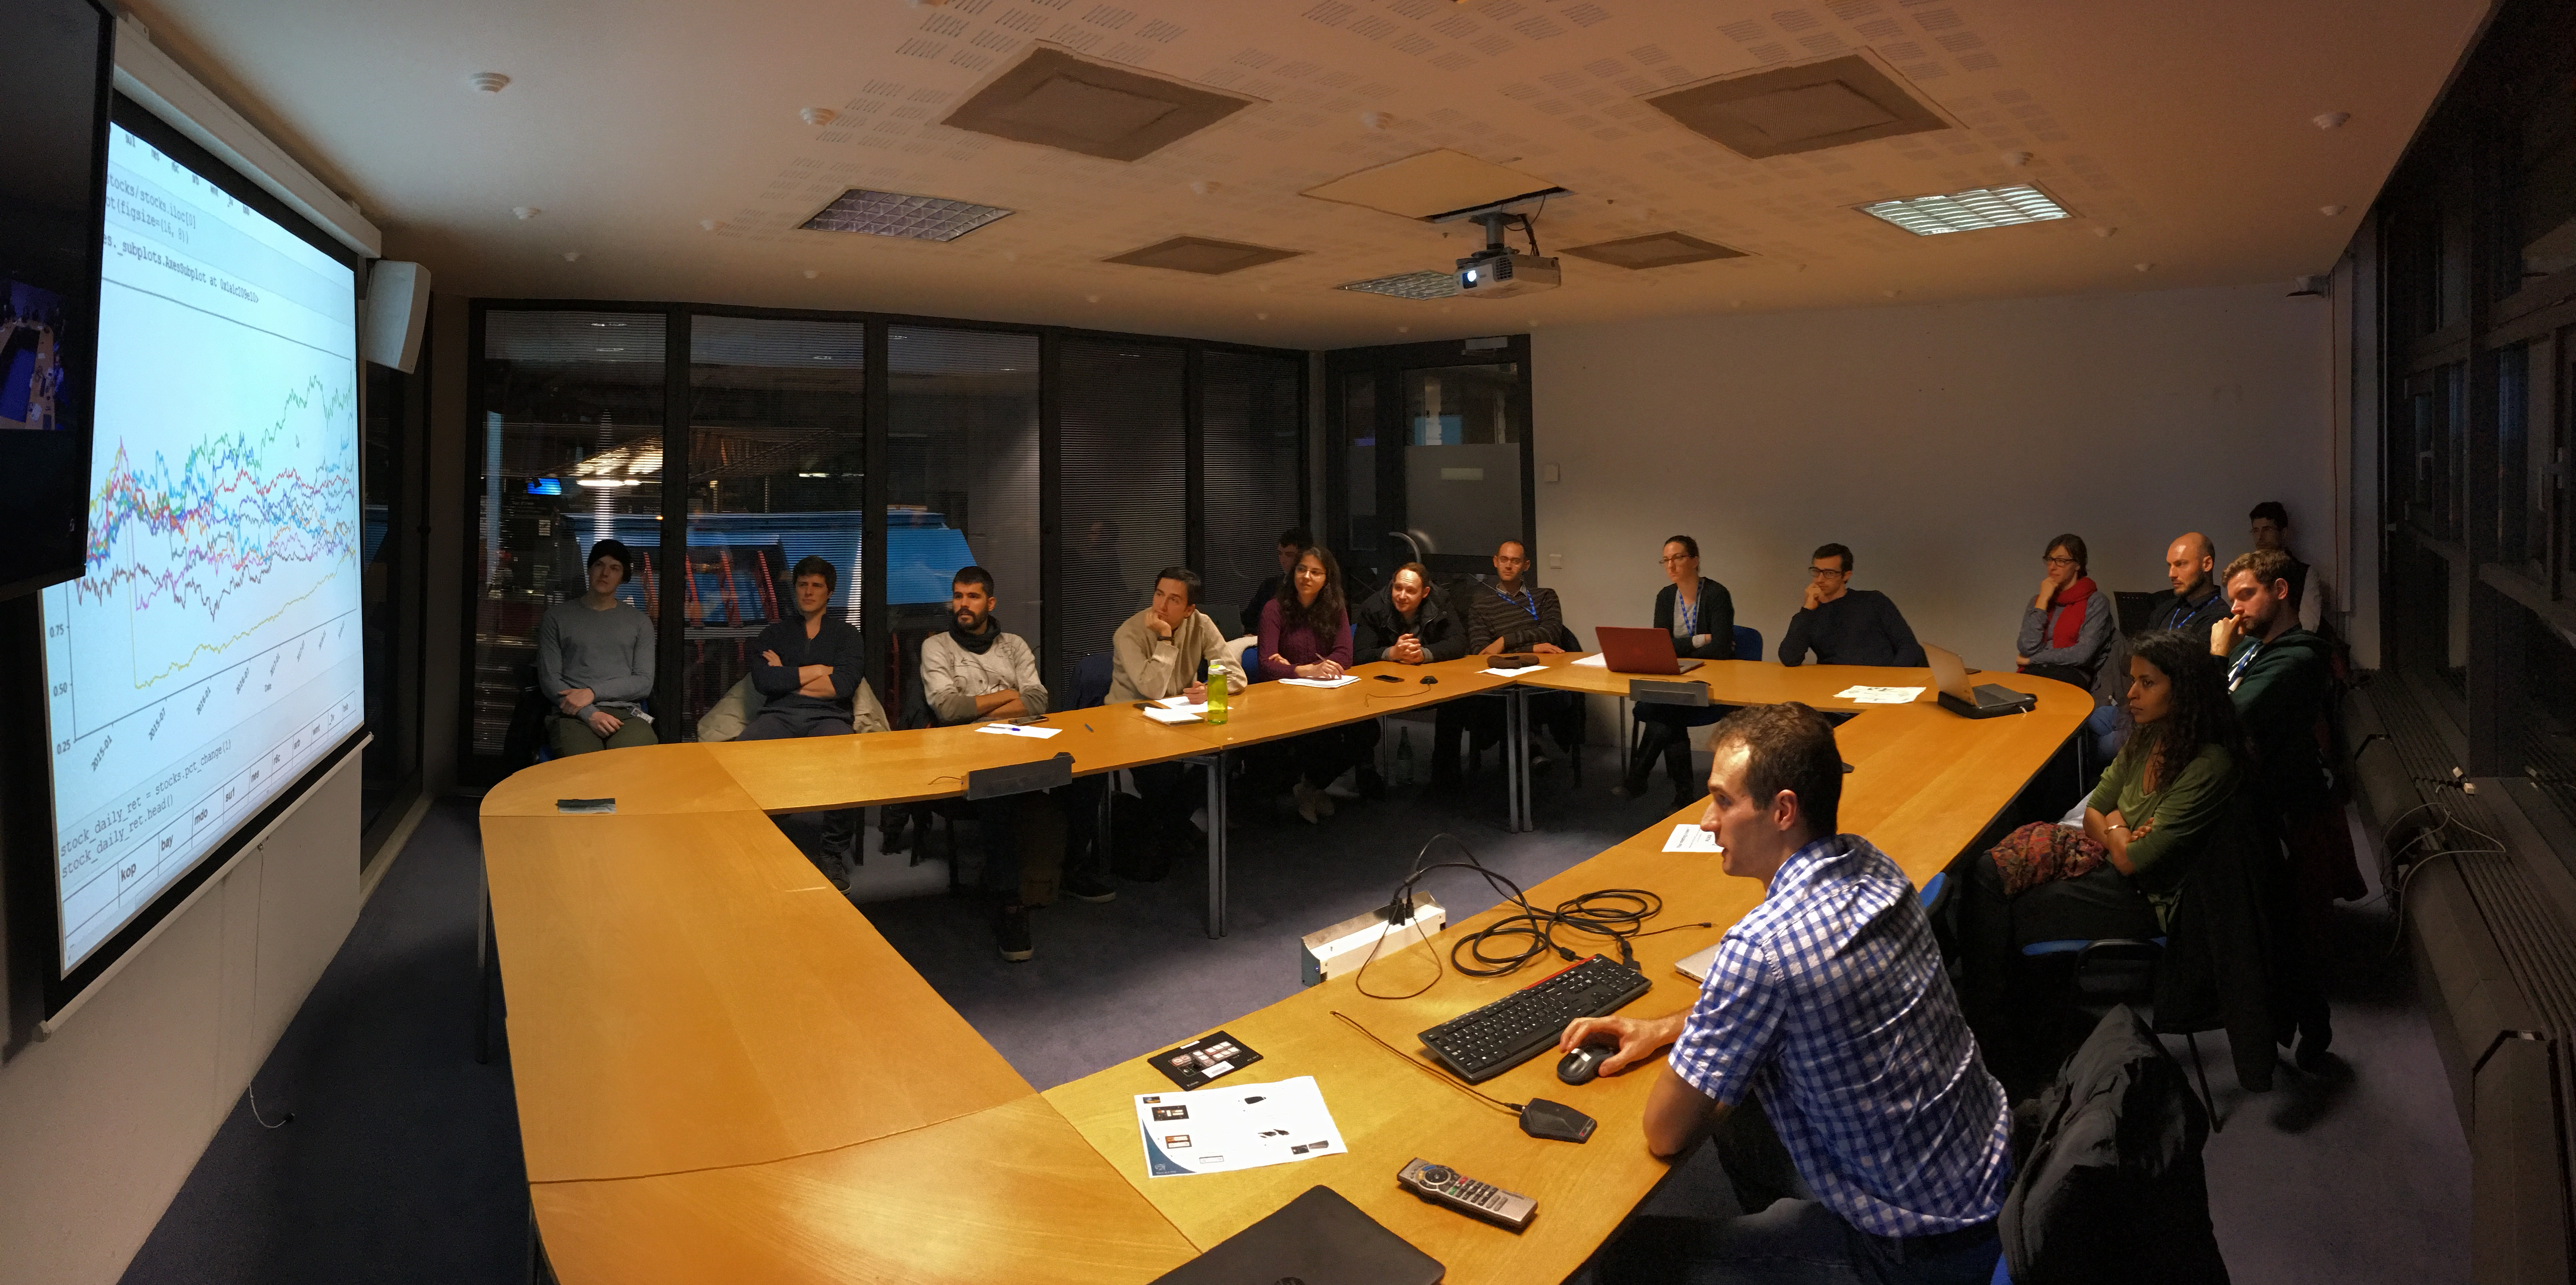
\includegraphics[width=0.54\textwidth]{finance2.jpg}\\
     \includegraphics[width=0.54\textwidth]{finance3}
     \includegraphics[width=0.54\textwidth]{boxing1.jpg}\\  
     \includegraphics[width=0.54\textwidth]{boxing2}
     \includegraphics[width=0.54\textwidth]{boxing4.jpg}\\
    \caption{ Top row: visit at SM18 and S'Cool lab. Second row: invited talks at the Finance Club. Third row: moderator at the CERN Alumni Collisions and CERN Relay Race trophy. Bottom row: Boxing Club.}
    \label{outreach}
   \end{figure}
\fi


